%% Estructura principal para un reporte de Trabajos intersemanales CIRCAE %%
\documentclass[a4paper]{IEEEtran} %tamaño del papel y el tipo de transcripción que será IEEE
\usepackage[utf8]{inputenc} %el tipo de codificación que incluye símbolos como la tilde
\usepackage[spanish]{babel} % hacemos que nuestro documentación vaya en español
\usepackage{cite} % citas bibliográficas
\usepackage{graphicx} %gráficos, usaremos solo .jpg o .png con estándares que ya veremos
\usepackage{subfigure}
\usepackage{url}
\usepackage{amsmath} 
%%%%%%% codigo
\usepackage{color}
\definecolor{gray97}{gray}{.97}
\definecolor{gray75}{gray}{.75}
\definecolor{gray45}{gray}{.45}

\usepackage{listings}
\lstset{ frame=Ltb,
framerule=0pt,
aboveskip=0.5cm,
framextopmargin=3pt,
framexbottommargin=3pt,
framexleftmargin=0.4cm,
framesep=0pt,
rulesep=.4pt,
backgroundcolor=\color{gray97},
rulesepcolor=\color{black},
%
stringstyle=\ttfamily,
showstringspaces = false,
basicstyle=\small\ttfamily,
commentstyle=\color{gray45},
keywordstyle=\bfseries,
%
numbers=left,
numbersep=15pt,
numberstyle=\tiny,
numberfirstline = false,
breaklines=true,
}
% minimizar fragmentado de listados
\lstnewenvironment{listing}[1][]
{\lstset{#1}\pagebreak[0]}{\pagebreak[0]}

\lstdefinestyle{consola}
{basicstyle=\scriptsize\bf\ttfamily,
backgroundcolor=\color{gray75},
}

\lstdefinestyle{C}
{language=C,
}
%%%%%%%
\providecommand{\keywords}[1]{\textbf{\textit{Términos Clave---}} #1}
\begin{document}

\title{WILKINSON POWER DIVIDER SIMULATION}
\author{Hanan Ronaldo Quispe Condori, CIRCAE Student Member
\thanks{Este primer párrafo puede contener auspiciadores u organizaciones que colaboraron con la realización de esta parte del proyecto y mencionar de manera expecífica que papel puntual tuvieron en el proceso... "This work was supported in part by the U.S. Department of Commerce under Grant BS123456."}
\thanks{Los siguientes párrafos pueden contebner datos específicos de los autores del proyecto, por ejemplo "F. A. Author is with the National Institute of Standards and Technology, Boulder, CO 80305 USA (e-mail: author\@ boulder.nist.gov)"}
\thanks{NombreA1 ApellidoA1 ApellidoA2, was with Rice University, Houston, TX 77005 USA. He is now with the Department of Physics, Colorado State University, Fort Collins, CO 80523 USA (e-mail: author\@ lamar.colostate.edu).}
\thanks{NombreB1 ApellidoB1 ApellidoB2 is with the Electrical Engineering Department, University of Colorado, Boulder, CO 80309 USA, on leave from the National Research Institute for Metals, Tsukuba, Japan (e-mail: author\@ nrim.go.jp).}}

\markboth{INFORME CIRCAE 2019-08-05-G1-P3-001}{} % Codigo del informe que corresponde a: semestre | mes | dia | numero de grupo con la G antepuesta | numero de proyecto con la P antepuesta | número de informe
\maketitle


\begin{abstract}
MicroMouse es un dispositivo en el que se aplica principios de ciencias de la computación, principios ópticos, mecánicos, electrónicos y la integración de tecnologías de software y hardware. Lo que se pretende cubrir es la solución de un laberinto usando algoritmos de reconocimiento, almacenamiento, solución y retroalimentación con condiciones iniciales constantes en el tiempo.\\
\keywords{\textbf{Introducimos nuestros términos clave en orden alfabetico, separado por comas. Para una lista de sugerencias de palabras o términos clave visitar \underline{http://www.ieee.org/organizations/pubs/ani\_ prod/keywrd98.txt}}}
\end{abstract}
\section{Problema}
If your paper is intended for a conference, please contact your conference 
editor concerning acceptable word processor formats for your particular 
conference. 

IEEE will do the final formatting of your paper. If your paper is intended 
for a conference, please observe the conference page limits. 

\subsection{Concepto Principal}

El problema abarcará lo que se pretende resolver o se resolvió con el informe, se tiene que ser claro y conciso.

\subsection{Abbreviations and Acronyms}
Define abbreviations and acronyms the first time they are used in the text, 
even after they have already been defined in the abstract. Abbreviations 
such as IEEE, SI, ac, and dc do not have to be defined. Abbreviations that 
incorporate periods should not have spaces: write ``C.N.R.S.,'' not ``C. N. 
R. S.'' Do not use abbreviations in the title unless they are unavoidable 
(for example, ``IEEE'' in the title of this article).

\begin{figure}
    \centering
        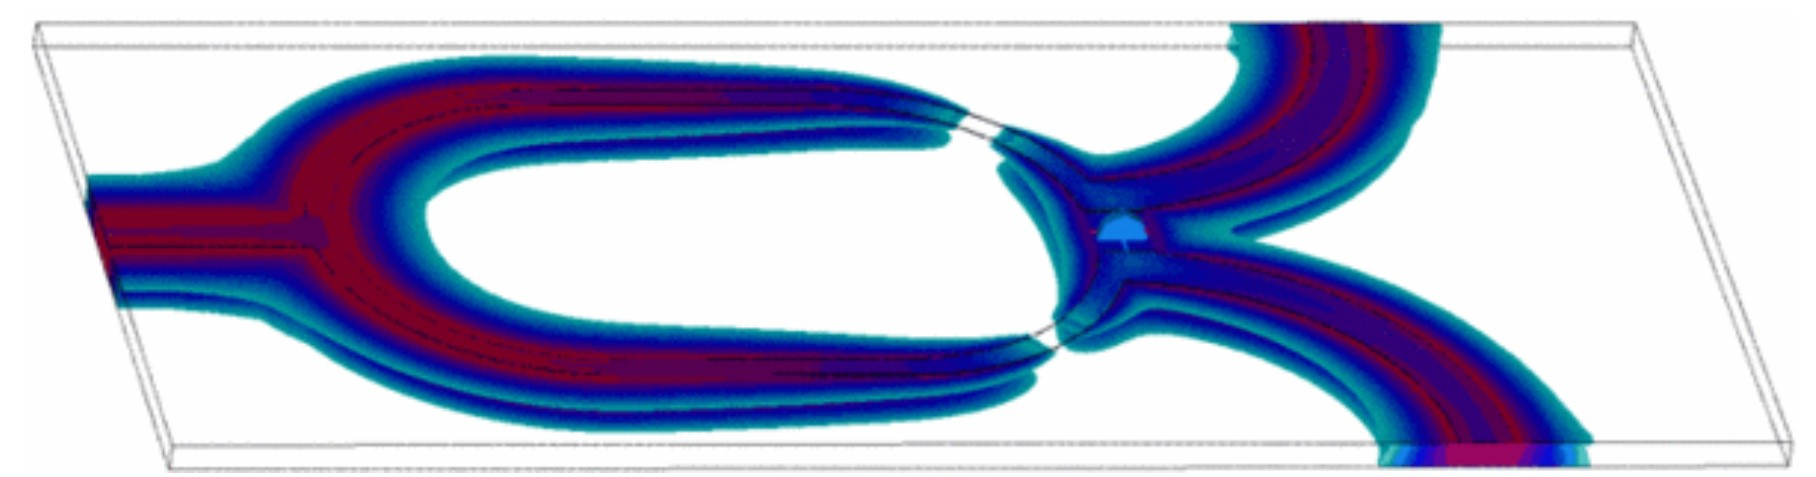
\includegraphics[width=8cm]{imagenes/img2}
        \caption{A gull}
        \label{fig:gull}
\end{figure}

\section{Objetivos}
Use either SI (MKS) or CGS as primary units. (SI units are strongly 
encouraged.) English units may be used as secondary units (in parentheses). 
This applies to papers in data storage. For example, write ``15 
Gb/cm$^{2}$ (100 Gb/in$^{2})$.'' An exception is when 
English units are used as identifiers in trade, such as ``3  
disk drive.'' Avoid combining SI and CGS units, such as current in amperes 
and magnetic field in oersteds. This often leads to confusion because 
equations do not balance dimensionally. If you must use mixed units, clearly 
state the units for each quantity in an equation.

The SI unit for magnetic field strength $H$ is A/m. However, if you wish to use 
units of T, either refer to magnetic flux density $B$ or magnetic field 
strength symbolized as $\mu _{0}H$. Use the center dot to separate 
compound units, e.g., ``A$\cdot $m$^{2}$.''

\subsection{Idea Principal}

Se plantea de manera general lo que se hará o se hizo para solucionar el problema.

\begin{equation}
 \left.\begin{aligned}
        B'&=-\partial \times E,\\
        E'&=\partial \times B - 4\pi j,
       \end{aligned}
 \right\}
 \qquad \text{Maxwell's equations}
\end{equation}

The word ``data'' is plural, not singular. The subscript for the 
permeability of vacuum $\mu _{0}$ is zero, not a lowercase letter 
``o.'' The term for residual magnetization is ``remanence''; the adjective 
is ``remanent''; do not write ``remnance'' or ``remnant.'' Use the word 
``micrometer'' instead of ``micron.'' A graph within a graph is an 
``inset,'' not an ``insert.'' The word ``alternatively'' is preferred to the 
word ``alternately'' (unless you really mean something that alternates). Use 
the word ``whereas'' instead of ``while'' (unless you are referring to 
simultaneous events). Do not use the word ``essentially'' to mean 
``approximately'' or ``effectively.'' Do not use the word ``issue'' as a 
euphemism for ``problem.'' When compositions are not specified, separate 
chemical symbols by en-dashes; for example, ``NiMn'' indicates the 
intermetallic compound Ni$_{0.5}$Mn$_{0.5}$ whereas 
``Ni--Mn'' indicates an alloy of some composition 
Ni$_{x}$Mn$_{1-x}$.

\section{Planteamiento/Procedimiento}
\label{sec:guidelines}

\subsection{Types of Graphics}
The following list outlines the different types of graphics published in 
IEEE journals. They are categorized based on their construction, and use of 
color/shades of gray:

\begin{figure}
    \centering
        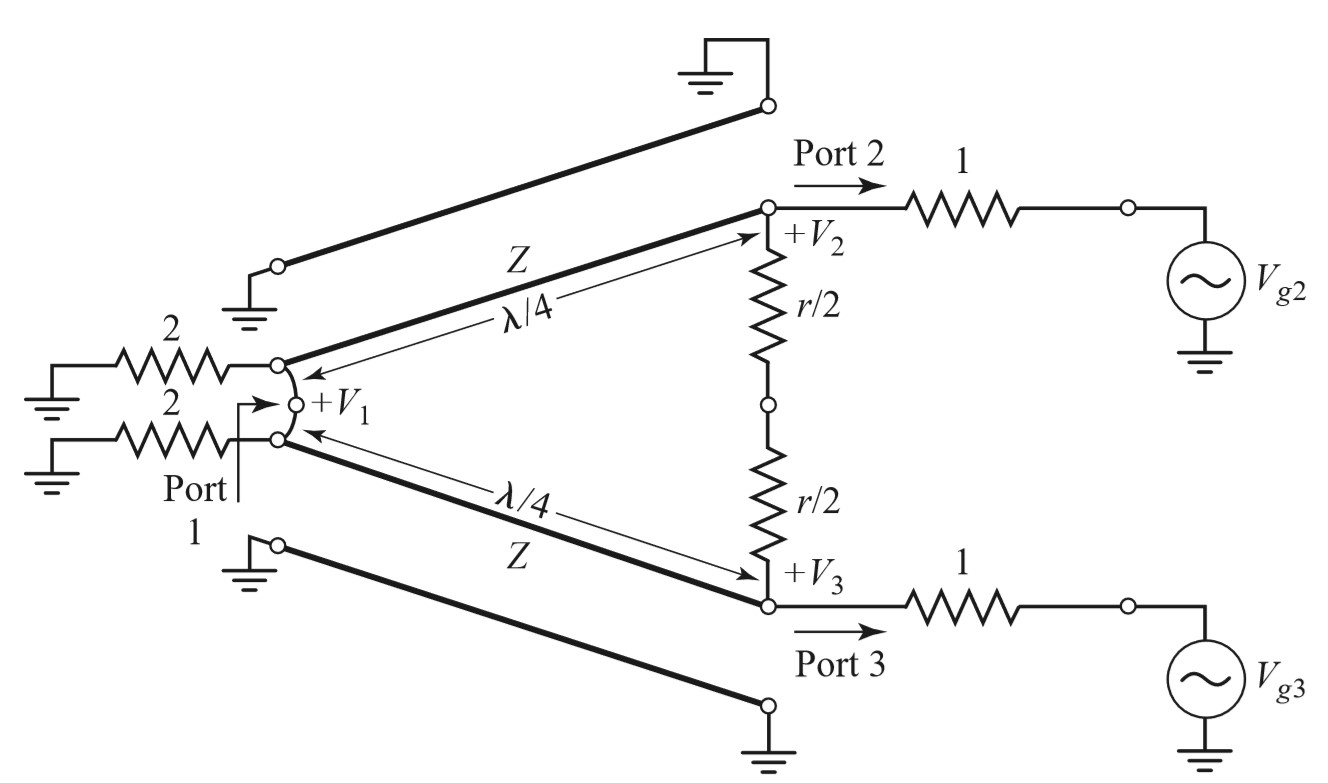
\includegraphics[width=8cm]{imagenes/img3}
        \caption{A gull}
        \label{fig:gull}
\end{figure}

\subsubsection{Color/Grayscale figures}
{Figures that are meant to appear in color, or shades of black/gray. Such 
figures may include photographs, illustrations, multicolor graphs, and 
flowcharts.}



\subsubsection{Line Art figures}
{Figures that are composed of only black lines and shapes. These figures 
should have no shades or half-tones of gray, only black and white.}

\begin{figure}
    \centering
        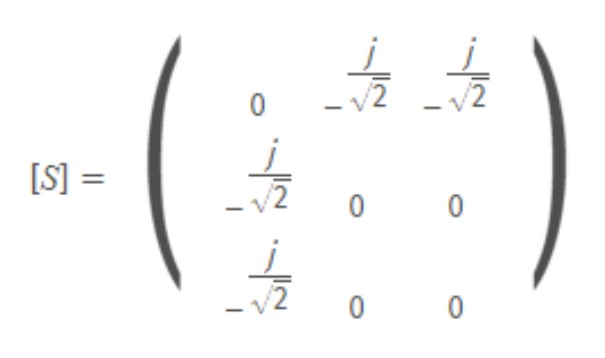
\includegraphics[width=8cm]{imagenes/img1}
        \caption{A gull}
        \label{fig:gull}
\end{figure}

\subsubsection{Author photos}
{Head and shoulders shots of authors that appear at the end of our papers. }

\subsection{Lineas de código}

\begin{lstlisting}[style=C]
import numpy as np
class NeuralNetwork:
  def __init__(self,
      no_of_in_nodes,
      no_of_out_nodes,
      no_of_hidden_nodes,
      learning_rate):
    self.no_of_in_nodes = no_of_in_nodes
    self.no_of_out_nodes = no_of_out_nodes
    self.no_of_hidden_nodes = no_of_hidden_nodes
    self.learning_rate = learning_rate
    self.create_weight_matrices()

  def create_weight_matrices(self):
    rad = 1 / np.sqrt(self.no_of_in_nodes)
    X = truncated_normal(mean=0, sd=1, low=-rad, upp=rad)
    self.weights_in_hidden = X.rvs((self.no_of_hidden_nodes,
         self.no_of_in_nodes))
    rad = 1 / np.sqrt(self.no_of_hidden_nodes)
    X = truncated_normal(mean=0, sd=1, low=-rad, upp=rad)
    self.weights_hidden_out = X.rvs((self.no_of_out_nodes,
         self.no_of_hidden_nodes))


  def train(self):
    pass

  def run(self):
    pass


if __name__ == "__main__":
  simple_network = NeuralNetwork(no_of_in_nodes = 3,
                   no_of_out_nodes = 2,
                   no_of_hidden_nodes = 4,
                   learning_rate = 0.1)
  print(simple_network.weights_in_hidden)
  print(simple_network.weights_hidden_out)
\end{lstlisting}

\noindent
Ahora compila usando \texttt{gcc}:

\begin{listing}[style=consola, numbers=none]
$ gcc  -o hello hello.c
\end{listing}

\subsubsection{Tables}
{Data charts which are typically black and white, but sometimes include 
color.}

\begin{table}
\caption{Units for Magnetic Properties}
\label{table}
\setlength{\tabcolsep}{3pt}
\begin{tabular}{|p{25pt}|p{75pt}|p{115pt}|}
\hline
Symbol& 
Quantity& 
Conversion from Gaussian and \par CGS EMU to SI $^{\mathrm{a}}$ \\
\hline
$\Phi $& 
magnetic flux& 
1 Mx $\to  10^{-8}$ Wb $= 10^{-8}$ V$\cdot $s \\
$B$& 
magnetic flux density, \par magnetic induction& 
1 G $\to  10^{-4}$ T $= 10^{-4}$ Wb/m$^{2}$ \\
$H$& 
magnetic field strength& 
1 Oe $\to  10^{3}/(4\pi )$ A/m \\
$m$& 
magnetic moment& 
1 erg/G $=$ 1 emu \par $\to 10^{-3}$ A$\cdot $m$^{2} = 10^{-3}$ J/T \\
$M$& 
magnetization& 
1 erg/(G$\cdot $cm$^{3}) =$ 1 emu/cm$^{3}$ \par $\to 10^{3}$ A/m \\
4$\pi M$& 
magnetization& 
1 G $\to  10^{3}/(4\pi )$ A/m \\
$\sigma $& 
specific magnetization& 
1 erg/(G$\cdot $g) $=$ 1 emu/g $\to $ 1 A$\cdot $m$^{2}$/kg \\
$j$& 
magnetic dipole \par moment& 
1 erg/G $=$ 1 emu \par $\to 4\pi \times  10^{-10}$ Wb$\cdot $m \\
$J$& 
magnetic polarization& 
1 erg/(G$\cdot $cm$^{3}) =$ 1 emu/cm$^{3}$ \par $\to 4\pi \times  10^{-4}$ T \\
$\chi , \kappa $& 
susceptibility& 
1 $\to  4\pi $ \\
$\chi_{\rho }$& 
mass susceptibility& 
1 cm$^{3}$/g $\to  4\pi \times  10^{-3}$ m$^{3}$/kg \\
$\mu $& 
permeability& 
1 $\to  4\pi \times  10^{-7}$ H/m \par $= 4\pi \times  10^{-7}$ Wb/(A$\cdot $m) \\
$\mu_{r}$& 
relative permeability& 
$\mu \to \mu_{r}$ \\
$w, W$& 
energy density& 
1 erg/cm$^{3} \to  10^{-1}$ J/m$^{3}$ \\
$N, D$& 
demagnetizing factor& 
1 $\to  1/(4\pi )$ \\
\hline
\multicolumn{3}{p{251pt}}{Vertical lines are optional in tables. Statements that serve as captions for 
the entire table do not need footnote letters. }\\
\multicolumn{3}{p{251pt}}{$^{\mathrm{a}}$Gaussian units are the same as cg emu for magnetostatics; Mx 
$=$ maxwell, G $=$ gauss, Oe $=$ oersted; Wb $=$ weber, V $=$ volt, s $=$ 
second, T $=$ tesla, m $=$ meter, A $=$ ampere, J $=$ joule, kg $=$ 
kilogram, H $=$ henry.}
\end{tabular}
\label{tab1}
\end{table}

\subsection{Multipart figures}
Figures compiled of more than one sub-figure presented side-by-side, or 
stacked. If a multipart figure is made up of multiple figure
types (one part is lineart, and another is grayscale or color) the figure 
should meet the stricter guidelines.

\subsection{File Formats For Graphics}\label{formats}
Format and save your graphics using a suitable graphics processing program 
that will allow you to create the images as PostScript (PS), Encapsulated 
PostScript (.EPS), Tagged Image File Format (.TIFF), Portable Document 
Format (.PDF), Portable Network Graphics (.PNG), or Metapost (.MPS), sizes them, and adjusts 
the resolution settings. When 
submitting your final paper, your graphics should all be submitted 
individually in one of these formats along with the manuscript.

\begin{equation}
\frac{\partial u}{\partial t}
   = h^2 \left( \frac{\partial^2 u}{\partial x^2}
      + \frac{\partial^2 u}{\partial y^2}
      + \frac{\partial^2 u}{\partial z^2} \right)
\end{equation}


\section{Conclusiones}
A conclusion section is not required. Although a conclusion may review the 
main points of the paper, do not replicate the abstract as the conclusion. A 
conclusion might elaborate on the importance of the work or suggest 
applications and extensions. 


%La bibliografía:
\bibliographystyle{ieeetr}
\bibliography{bibliografia}

\end{document}